\chapter{引言}
\label{chap:introduction}

% Sec 1.1
\section{研究背景与意义}
\label{sec:background}
计算流体力学 (Computational Fluid Dynamics, CFD) 是一个应用数值方法对流体力学问题求解,以预测流场动态的学科。从20世纪后半叶学科建立至今,其已发展成为一门成熟的、横跨流体力学、数值分析、偏微分方程数值理论与计算机科学等多个领域的交叉学科,并在生产实践中发挥日益重要的作用。计算流体力学最先被应用于航空航天领域,但现在已经成为了汽车、舰船、列车乃至风力涡轮机和风力发电厂设计中不可或缺的一环~\citep{https://doi.org/10.1002/we.458}。图~\ref{img:cfd_impact_on_planes} 展示了波音 (Boeing) 在最新的飞机设计中对计算流体力学的广泛使用。而随着小型机及个人电脑的出现,计算成本的降低使得计算流体力学所发展的流体仿真技术得以应用至更多领域,并带动相关学科的发展,其中一个典型的例子就是气动声学 (aeroacoustics)。1992年气动声学领域的开创者詹姆斯·莱特希尔 (James Lighthill) 预言计算机仿真会为气动声学带来第二个黄金时代~\citep{hardin1993computational}。随后,计算气动声学 (Computational Aeroacoustics, CAA) 学科作为气动声学的分支开始建立,以使用数值方法分析湍流产生的噪声。随着人们对噪声问题的愈发关注,计算气动声学已成为研究噪声源、噪声产生机理和控制方法的一类主要方法~\citep{RN177}。

\begin{figure}[htbp]
    \centering
      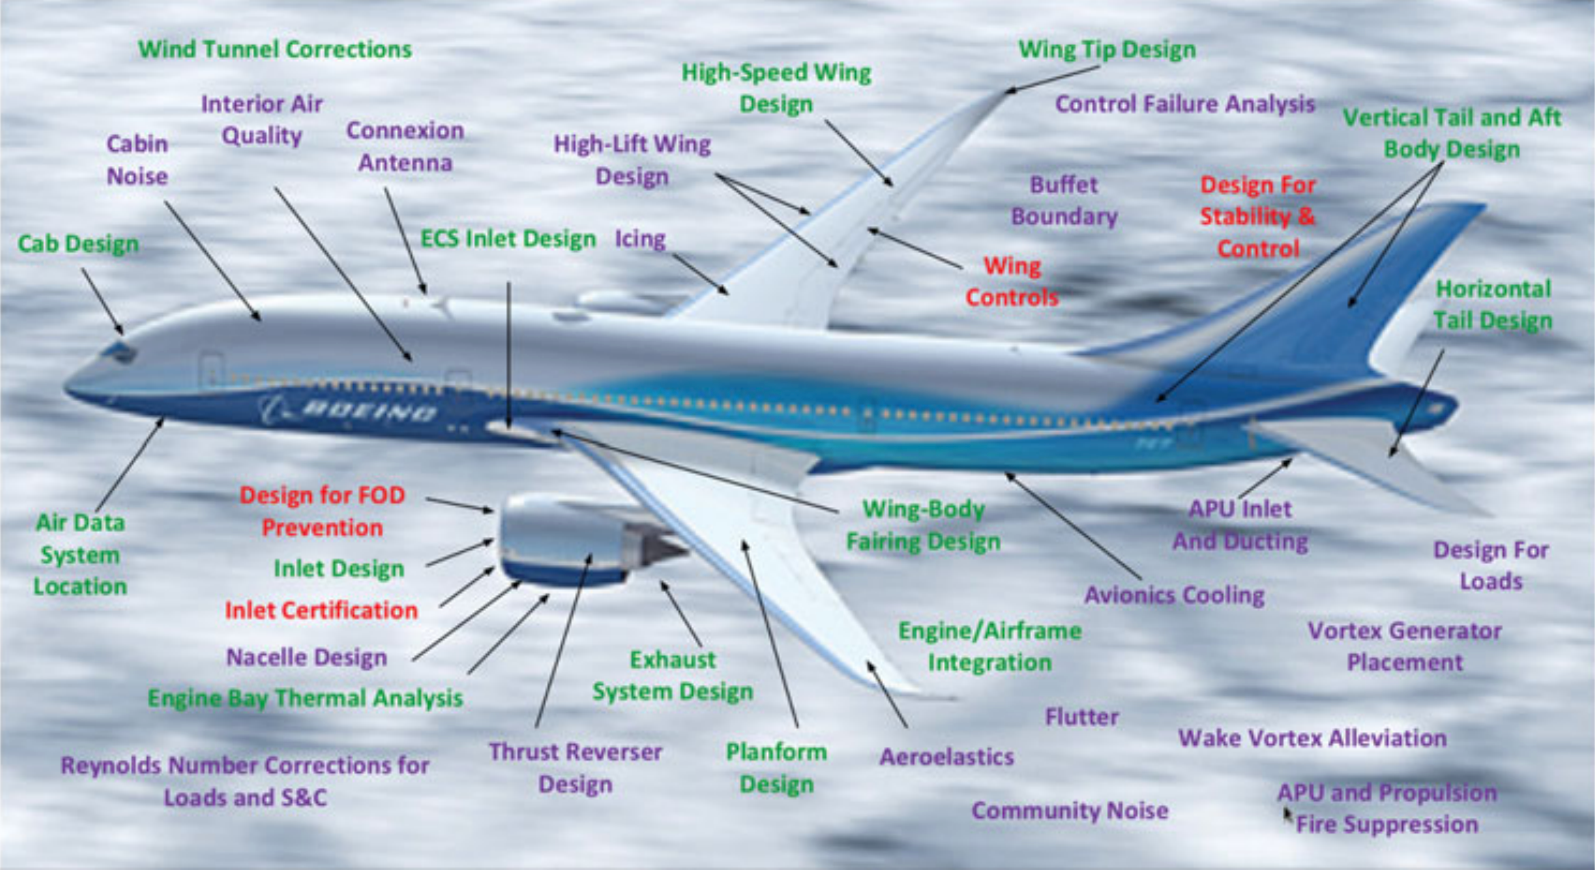
\includegraphics[width=0.99\columnwidth]{figures/cfd_impact_on_planes.png}
    \bicaption[计算流体力学在飞机设计中的作用]{计算流体力学在飞机设计中的作用。绿色表示计算流体力学对该部分的设计有较强影响,紫色表示有部分影响,红色表示有应用潜力。图片来自~\citep{spalart_venkatakrishnan_2016}。}{CFD influence on aircraft design. The green areas have a strong impact, purple areas have some impact, and the opportunities for the future are in red. Image from~\citep{spalart_venkatakrishnan_2016}.}
    \label{img:cfd_impact_on_planes}
\end{figure}

随着技术与需求的发展,流体仿真也不再是一个纯粹用于工程应用和分析的技术,如在娱乐工业中,流体仿真也有着举足轻重的地位。20世纪90年代,基于物理的流体动画 (physically-based fluid animation) 技术开始在计算机图形学 (Computer Graphics, CG) 中出现,并之后被广泛应用于娱乐工业的游戏及视觉特效制作中。其中有多个流体仿真技术由于其对电影产业的杰出贡献获得奥斯卡技术成就奖 (Academy Award for Technical Achievement),包括Maya“流体效果” (Fluid Effects) 系统、工业光魔 (Industrial Light \& Magic, ILM) 的Plume流体仿真系统 (见图~\ref{img:star_wars}) 等。相比计算流体力学更多关注计算精度和问题本质,视觉特效则需要复杂效果和表现力~\citep{C1}。这也使得两个领域的流体仿真方法一定程度上有所分化。

\begin{figure}[htbp]
  \centering
    
\includegraphics[width=0.99\columnwidth]{figures/star_wars.png}
  \bicaption[流体仿真技术在电影工业中的运用]{流体仿真技术在电影工业中的运用。图中展示了《星球大战:最后的绝地武士》(Star Wars: The Last Jedi) 影片中一些通过仿真得到的特效镜头,这些仿真由工业光魔的Plume流体仿真系统实现,该系统在2014年获得奥斯卡技术成就奖。图片来自~\citep{10.1145/3214745.3214778}。}{Application of fluid simulation technique in motion picture industry. The figure demonstrates some effects simulation shots in Star Wars: The Last Jedi using ILM's Plume fluid simulation system, for which ILM received the Academy Award for Technical Achievement in 2014. Image from~\citep{10.1145/3214745.3214778}.}
  \label{img:star_wars}
\end{figure}

现有的流体仿真技术虽被广泛地应用于多个领域,但其依然存在许多缺陷。目前主流的流体仿真方法依然是从宏观层面对纳维-斯托克斯 (Navier-Stokes, N-S) 方程进行求解,这些方法的一个主要问题是很难以合理的计算成本获得足够精确的解。如求解层流与湍流的过渡、湍流的流场动态、湍流的边界层分离等问题时,获得的解的精度与计算成本是非常相关的。美国国家航空航天局 (National Aeronautics and Space Administration, NASA) 最近的一项研究就突出了高性能计算 (High-Performance Computing, HPC) 平台对现今CFD在航空航天应用中的重要性~\citep{slotnick2014cfd}。而随着新的硬件架构,如图形处理单元 (Graphics Processing Unit, GPU),的算力提升,其在科学计算中的应用也越来越广泛。GPU架构相比传统HPC平台中的处理器架构,可以大幅降低并行代码的运行时间,从而提升计算效率。然而目前的不可压N-S求解器中需要求解泊松 (Poisson) 方程,这样的全局求解会大幅降低GPU的计算效率,也是传统流体仿真方法应用于GPU架构的一大阻碍。

面临这种物理精度与性能之间的矛盾,计算机图形学中的流体仿真方法更多倾向于在保证视觉真实感的前提下提升效率。除了使用自适应网格或硬件加速等常规方法外,典型的提升效率的方法还包括使用简化模型~\citep{doi.org/10.1111/cgf.12825} 或数据驱动方法~\citep{10.1145/2816795.2818129},在粗糙网格下添加高精度细节,如湍流合成~\citep{10.1145/1360612.1360649}和多层次解算~\citep{10.1145/1833349.1778785}等。但这些方法较大程度地牺牲了物理精度,以保证求解的效率,且很多方法只可应用于某一个具体场景下的流体仿真,并不能成为较为通用的流体仿真方法。

此外,传统的CFD方法对几何网格与计算网格的质量要求都十分严格。在FVM这类方法中,不满足要求的几何网格经常会造成流体仿真结果的发散。在工业制造领域 (如汽车工业),人工制作这样的网格可能需要工程师数日的时间,对于整体的仿真效率有很大影响。同时,对于所有基于网格的流体仿真方法,计算网格的细化都是十分重要的。一方面,由于实际应用中解算的物理尺度可能很大,网格细化可以有效地节省计算资源。另一方面,我们解算时使用的计算域一般会比实际我们感兴趣的区域大上很多,以避免计算域边界对流体结构产生影响~\citep{coreixas2015round, doi:10.2514/6.2015-2993}。这需求我们在对流体有关键影响的区域使用更高的空间分辨率,而构建符合要求的多分辨率网格也十分繁琐。如何高效、自动化地构建自适应计算网格,也是提升仿真效率与精度的关键问题。

针对这些问题,格子玻尔兹曼方法 (Lattice Boltzmann Method, LBM) 作为一个较为新颖的流体仿真方法,开始受到重视。从该方法被提出~\citep{PhysRevLett.61.2332} 至今三十多年的时间过去,其求解流体的能力不断被发展和验证,并成为一个可以替代传统的求解N-S方程的流体仿真方法~\citep{ARUMUGAPERUMAL2015955}。LBM通过求解格子玻尔兹曼方程 (Lattice Boltzmann Equation, LBE),从介观层面 (即微观粒子在统计上的分布) 进行流体仿真。在这一过程中,LBM的时间步是显式推进的,且无需求解全局方程,非线性的碰撞项只需要空间上的局部求解,这一点使得LBM非常适合大规模并行计算。并且,LBE只包含一阶偏微分方程,而N-S方程则包含二阶偏微分方程。这不仅使LBM的实现更简洁,也使LBM相比传统的N-S方法有着更高的求解效率与更低的数值误差。在理论精度上,LBE可以通过查普曼-恩斯科格 (Chapman-Enskog) 分析与N-S方程建立联系,从而证明LBE在弱可压流体中,与N-S方程在宏观上等同~\citep{Y.H.Qian_1993}。这保证了LBM的理论精度。

LBM的另一独特优势为,LBM对低速 (马赫数低于0.3) 的可压缩非稳态湍流求解非常高效,所以可以直接通过仿真计算亚声速情况下的气动声。这样的直接噪声计算 (Direct Noise Computation,DNC) 在使用传统N-S方法时是十分困难的,因为在湍流情况下对可压缩非稳态N-S方程求解的计算成本是巨大的。虽然可以求解雷诺平均纳维-斯托克斯 (Reynolds-Averaged Navier-Stokes, RANS) 方程得到平均流场后,再结合莱特希尔 (Lighthill) 方程~\citep{doi:10.1098/rspa.1952.0060} 与FW-H (Ffowcs Williams-Hawkings) 声比拟积分法~\citep{doi:10.1098/rsta.1969.0031} 进行声场传播求解 (这也被称为CAA中的混合方法)。但是显然,平均流场信息中高频信号是丢失的,这样的混合方法相比直接噪声计算精度有所下降。而LBM的高效湍流求解使得LBM成为计算气动声学领域的一个非常有前景的直接仿真方法。高精度、高效率和实现简洁的优势使得LBM有着同时满足工业制造、气动声分析与视觉动画等不同领域需求的潜力。

但同时,在技术层面格子玻尔兹曼方法也有一些亟待解决的问题。第一点是亚网格物体的流固耦合问题。亚网格物体是指某些维度远小于计算网格大小的物体。由于这些网格亚网格的特点,它们的几何特征很难被一般的流固耦合方法捕捉,从而会造成错误的求解结果。第二点是边界处理及碰撞模型的精度及稳定性不足。虽然LBM在很多验证案例中都有着优秀的精度表现,但一些极难使用数值仿真复现的物理现象 (如高雷诺数下的湍流边界层分离) 对于LBM也依然具有挑战。这样问题的本质是LBM中的碰撞模型与边界处理的精度与稳定性还有待进一步提升。第三点是计算网格构建复杂的问题。因为LBM大多使用笛卡尔网格作为计算网格,所以对几何网格的质量要求相比传统N-S方法是大幅降低的。但是对于计算网格,LBM同样缺乏高效、自动化的多分辨率网格构建手段。

为了解决这一系列问题,本文基于现有的格子玻尔兹曼方法,提升其求解精度和稳定性,构建了整体的流体仿真框架,以自动化地完成高效、高精度地流体仿真,并展示其在不同领域中的应用。首先,针对亚网格物体的流固耦合问题,本文提出了基于速度修正和简单反弹 (Simple Bounce-Back, SBB) 边界方法的混合边界方法。该方法可以求解流体与轻薄物体的交互,如薄片、细棒等。这些物体的某些尺度通常比仿真域的离散尺度还要小,在传统的流体仿真方法中极易引起流体泄露。本文提出的新的混合边界方法在解决流体泄露问题的同时,提升了求解的稳定性。其次,针对于需要更高精度的应用,本文还提出了新的单点插值反弹 (Interpolated Bounce-Back, IBB) 边界方法,与基于熵优化的累积量碰撞模型。通过与物理实验的比较,本文验证了新的方法相比现有方法有着进一步的精度提升,并可以模拟出物理上的阻力危机现象。在实现与效率上,本文提出了基于距离场的自动计算网格构建方法,该方法可以自动识别出有效的流体区域,并依据与固体距离的远近自动细分网格,实现了快速、简便的网格生成。最后,本文提出了整个框架的GPU优化算法,在代码层面进一步提升运行效率。

在技术层面之外,我们也注意到LBM本身由于其发展时间较短,在许多领域并没有得到足够的关注。如在本文中的工作提出之前,计算机图形学中仅有非常少量的工作使用LBM进行湍流气体仿真~\citep{10.1109/TVCG.2012.303, Li-2019, Li-2020},在CFD领域使用LBM进行超高雷诺数湍流仿真 ($Re>100,000$) 的应用也较为有限~\cite{10.1063/5.0046938}。而本文的核心目标为进一步提升LBM方法的精度、稳定性与易用性,将其应用至图形学仿真的同时,推动LBM在计算流体力学、计算气动声学等不同领域中的发展与应用,缩小这些不同领域中计算方法的区别,提出一个统一、高效、精准的流固耦合仿真框架,并完善相关实现方法,使流体仿真技术在现实中有着更强的指导意义。


% Sec 1.2
\section{研究现状}
本章节将三个方面介绍相关研究工作。首先于第~\ref{sec:1_related_works_CFD} 节回顾计算流体力学领域中的流体仿真方法,之后于第~\ref{sec:1_related_works_CG} 节回顾计算机图形学领域中的流体仿真方法,最后于第~\ref{sec:1_related_works_LBM} 节介绍LBM方法中相关技术的发展。

% Sec 1.2.1
\subsection{计算流体力学中的流体仿真方法}
\label{sec:1_related_works_CFD}
\paragraph{有限差分方法}
有限差分方法是最简单而易于实现的偏微分方程求解方法。应用于N-S方程时,有限差分方法同样只需要较小的计算量即可求解~\citep{kooij2018comparison,vreman2014comparison}。但是只有极少数情况中,有限差分方法被应用于湍流仿真。在求解不可压缩N-S方程时,需要额外求解全局的泊松方程来满足不可压条件 (使速度场散度为0),这也是使用有限差分方法进行流体仿真的难点。对于拉普拉斯算子 (Laplace operator),通常需要使用迭代的求解方法 (如多重网格方法~\citep{golub2013matrix}) 来求解线性系统。其次,对于非线性平流项,有限差分方法往往采取半拉格朗日方法~\citep{smolarkiewicz1992class}。但这会带来很大的数值黏度误差。现代CFD中比较重要的差分格式为总变差减小 (Total Variation Diminishing, TVD) 格式~\citep{osher1986very, YEE1985327, HARTEN1983357}。在TVD格式中,已经通过对左右模板 (stencil) 的导数值的比较来进行自适应的选择适当的值,这一思想也被扩展到了之后的基本无震荡 (Essentially Non-Oscillatory, ENO) 格式~\citep{HARTEN19973, SHU198932, SHU1988439}与加权基本无震荡 (Weighted Essentially Non-Oscillatory, WENO) 格式~\citep{LIU1994200}。但是由于有限差分方法在多维问题上只能在各个维度上进行一维近似,所以其只能应用于结构化网格,从而对复杂几何体的处理能力有限。

\paragraph{有限体积方法}
相对于有限差分方法从微分形式的方程出发,有限体积方法通过从积分形式的方程出发出发构造算法,这使得有限体积方法有着天然的守恒性。也因为它直接计算积分项,使其可以直接应用于非结构网格上。这些特点使得有限体积方法能够运用于复杂几何体的计算。目前,有限体积方法被广泛应用于商业流体仿真软件中,如Ansys FLUENT,Ansys CFX等~\citep{JEONG201419}。 
对于不可压缩的流体,典型的显式有限体积法必须与压力投影阶段相结合,以得到无旋的速度场~\citep{https://doi.org/10.1002/fld.310, pember1996higher}。为了提高稳定性,对速度和压力进行离散时,通常会使用交错网格。虽然在结构化网格中实现这一点并不难,但非结构网格中这依然有一定的挑战~\citep{herbin2012staggered, gao2012unstructured, bermudez1998upwind}。此外,也有工作提出了更高阶的有限体积方法,如k-exact有限体积方法~\citep{barth1990higher}与WENO有限体积方法~\citep{HU199997}等。

\paragraph{有限元方法}
有限元方法将仿真域离散为许多小区域 (即有限元),每个单元可以看作是整个解的一个分段的近似。通过有限元方法求解偏微分方程通常先要将方程改写为弱形式,这个求解的方法称作伽辽金 (Galerkin) 方法。而因为其采用连续函数空间,使得每个单元之间无法完全独立,在求解时需要求解一个全局的庞大线性方程组,所需的计算消耗使得该方法并未在流体仿真领域得到广泛应用。而随后,间断伽辽金 (Discontinuous Galerki, DG) 方法被提出,最早其被用于求解中子运输方程~\citep{reed1973triangular},与龙格-库塔 (Runge-Kutta) 方法结合后被推广并应用到双曲守恒律方程的求解中~\citep{cockburn2001runge, cockburn1990runge, cockburn1989tvb2, cockburn1989tvb3}。在此之后该方法也开始被应用于CFD领域~\citep{Zienkiewicz-2013, lomtev1999discontinuous, bassi1997high}。为了改进DG方法计算量大等缺点,无积分型 (quadrature-dree) DG~\citep{atkins1998quadrature}与节点型 (nodal) DG~\citep{hesthaven2007nodal}也被相应提出。

% Sec 1.2.2
\subsection{计算机图形学中的流体仿真方法}
\label{sec:1_related_works_CG}
\paragraph{流体仿真方法}
相对于CFD领域中流体仿真对精度的追求,CG中的流体仿真方法更加注重效率与灵活性。例如早期~\citet{Stam-1999} 提出的简单的无条件稳定的半拉格朗日方法。该方法开创了CG领域流体仿真的研究,但该方法因为有较强的数值耗散误差而无法进行湍流的仿真。之后的许多工作提出了新的数值求解方法从而改善这一情况,如 前后误差补偿和校正 (Back and Forth Error Compensation Correction, BFECC) 方法~\citep{Kim-2005},无条件稳定的麦科马克 (MacCormack) 方法~\citep{Selle-2008},对流-反射 (advection-reflection) 方法~\citep{Zehnder-2018}与对流量双向映射(Bi-directional Mapping of convective quantities, BiMocq$^2$) 方法~\citep{Qu-2019}。但这些方法通常会带来额外的数值色散误差。
因为烟雾动画更加注重其表面涡量的模拟,涡方法应运而生。涡方法将N-S方程重新构造为了基于涡量的形式~\citep{Park-2005, Selle-2005},并使用涡丝~\citep{Weissmann-2010, Angelidis-2005}或涡片~\citep{Zhang-2015, Zhang-2014, Pfaff-2012}进行仿真。除去上述基于网格的方法,也有部分基于粒子的方法被应用于CG领域的流体仿真。如光滑粒子流体动力学 (Smoothed Particle Hydrodynamics, SPH) 由于其易于实现的特性与良好的视觉效果,是CG领域中十分流行的液体仿真方法~\citep{Ihmsen-2014-1, Becker-2007, Adams-2007, Muller-2003, Desbrun-1996}。为了更好地保证流体的不可压缩性,基于密度~\citep{Bender-2015, Ihmsen-2014-2, Solenthaler-2009}或空间位置~\citep{Macklin-2013}的修正被提出以改善SPH方法的视觉效果。
此外,还有混合方法尝试结合网格与粒子方法的优点~\citep{Zhu-2005, Foster-1996, Brackbill-1986, Harlow-1962}。基于此,有工作~\citep{Fu-2017, Jiang-2015}进一步通过更精准的网格与粒子间的转换提升了精度。近来,\citet{Fei-2021} 使用了分离的积分方法降低了数值耗散,\citet{Qu-2022} 提出了新的网格与粒子间的转换方法以更好的保证流体体积的一致性。

\paragraph{流固耦合方法}
早期的工作在流固耦合仿真时,会将固体看作拉格朗日方法中的离散点,使每个点在固体和流体中发挥不一样的作用。在流体中,每个点的速度对应为诺伊曼 (Neumann) 边界条件,这使得流体上会有受力,而在固体表面上则受到大小相同方向相反的压力~\citep{Carlson-2004,Genevaux-2003,Takahashi-2002,Foster:2001,Yngve:2000}。
这些方法的耦合有显式格式也有半隐式格式,之后使用完全隐式格式来耦合流体固体速度的方法也被提出~\citep{Klingner-2006,Chentanez:2006:SCP,Batty-2007}。\citet{Teng-2016} 提出了完全使用欧拉方法处理流固耦合的方法。近来,单一框架的方法~\citep{takahashi-2020,fang-2020}被提出以支持流固之间的双向强耦合,但由于计算的复杂性,这类方法只能处理较小的尺度。
相比于常见固体,与薄片耦合的流体仿真难度更大,大多数需要特殊处理,如单边的基于求交的修正以防止流体泄露,或进行两次压力求解以计算应用于固体上的耦合作用力~\citep{Guendelman-2005}。
也有方法提出了更精准的动量转移与虚拟单元方法~\citep{Robinson:2009, Robinson-2008}。理论上,基于自适应网格的欧拉方法~\citep{Elcott-2007,Klingner-2006,Feldman:DF:2005,Feldman-2005,dai-2005}或拉格朗日方法~\citep{Clausen-2013,Misztal:2010}可以处理任意形状的固体,但这些方法需要频繁地调整网格结构,从而降低计算效率。
为了降低计算难度,部分基于切削网格 (cut-cell) 的方法使用了类有限体积的形式,在单元内切割出贴合边界的区域以防止流体穿过物体~\citep{Azevedo-2016,Liu:2015:MVF,weber-2015,Edwards-2014,gibou-2012,Ng-2009,Batty-2007,Roble-2005}。
对于基于粒子的流体仿真方法,通常会在流体上施加惩罚力以实现边界条件~\citep{peer-2015,Ihmsen-2013}。\citet{Gao:2017} 在流体隐式粒子 (FLuid-Implicit-Particle, FLIP) 方法中加入了贴合物体形状的约束, 但该方法在湍流中有稳定性问题。并且,绝大部分的基于粒子的方法无法保证流体压力的一致性~\citep{band-2018}。
此外,也有部分混合方法,使用网格来完成耦合的同时,利用粒子进行流体仿真~\citep{Fei-2019,Fei-2018,hu-2018,Zhang-2016}。

% Sec 1.2.3
\subsection{格子玻尔兹曼方法}
经历了三十余年的发展,格子波尔兹曼方法在各个方面都有了长足的进步。其中碰撞模型与边界处理作为影响流体求解的核心因素,从LBM诞生开始就是研究人员关注的重点。而随着应用领域的扩展与精度要求的提升,大规模流体仿真所需的网格细化与高效迁移算法也成为了LBM不可或缺的部分。这里我们将从这四个方面主要回顾格子玻尔兹曼方法的相关工作。
\label{sec:1_related_works_LBM}
\paragraph{碰撞模型}
在LBM中最简洁也最易于实现的碰撞模型为BGK (Bhatnagar-Gross-Krook) 碰撞模型~\citep{Chen-1998, Bhatnagar-1954},然而在高雷诺数流体中,BGK模型有着很大的截断误差,从而在数值上非常不稳定。多松弛时间 (Multiple-Relaxation-Time, MRT) 碰撞模型~\citep{Coveney-2002, Lallemand-2000, dHumieres-1992}尝试通过在矩 (moment) 空间进行松弛,来提升整体的数值稳定性与准确性。最初MRT碰撞模型通过原始矩 (raw moment) 进行构造,而这一形式违反了伽利略不变性 (Galilean invariance)。而之后为了进一步提升精度与稳定性,基于中心矩 (central moment)~\citep{Geier-2006, Geier-2009}、埃尔米特矩 (Hermite moment)~\citep{Shan-2007, Chen-2014, Adhikari-2008}、中心埃尔米特矩 (central Hermite moment)~\citep{Mattila-2017, Shan-2019}和累积量 (cumulant)~\citep{Geier-2015, Geier-2017}的MRT碰撞模型被提出,并满足了伽利略不变性。
还有一类碰撞模型是对分布函数进行埃尔米特多项式 (Hermite polynomial) 展开后截断来去除非流体动力学的模态 (non-hydrodynamic modes),之后进行碰撞。这类碰撞模型被称为正则化 (regularized) 碰撞模型~\citep{Zhang-2006, Latt-2006}。后期有工作通过递归形式改进了正则化碰撞模型,被称为递归正则化碰撞模型~\citep{Malaspinas-2015, Coreixas-2017}。作者证明了该方法有着更好的数值耗散和色散性质。\citet{Jacob-2018} 之后又提出了混合递归正则化模型,对二阶应力张量的重构做了调整,提高了方法的稳定性。
另一类对碰撞模型的改进路线是动态调整松弛时间,主要的方法包括大涡模拟 (Large-Eddy Simulation, LES) 亚网格模型~\citep{Eggels-1996, Sagaut-2010}和基于熵优化的碰撞模型~\citep{Karlin-1999, Ansumali-2003}。
对于LES亚网格模型,在LBM中最早被应用的是斯马古林斯基 (Smagorinsky) 模型~\citep{Hou-1994, Krafczyk-2003}。之后的工作通过包含动态的参数估计~\citep{Premnath-2009}、范德里斯 (van Driest) 阻尼函数~\citep{Malaspinas-2014}与改进的应力项~\citep{Leveque-2007},来提升壁面流体描述的精度。
除了使用涡流黏度之外,还有基于近似反卷积的模型~\citep{Malaspinas-2011, Nathen-2018}和壁面自适应大涡模型 (Wall-Adaptive Large Eddy, WALE)~\citep{Weickert-2010}被应用在LBM中。
同时,基于熵优化的碰撞模型通过最大化局部熵值,为高阶矩的松弛时间提供了一个有效的约束。然而,在碰撞过程中求解带约束的熵优化问题在数值上耗费很大。所以有不少方法尝试优化求解效率,如KBC (Karlin-B\"osch-Chikatamarla) 模型~\citep{Karlin-2014}、基于伪熵的方法~\citep{Kramer-2019}和使用解析解进行优化的方法~\citep{Tang-2022}。
除了亚网格模型与熵优化之外,近来也有方法通过离线的回归方法来优化松弛时间~\citep{Li-2020}。

\paragraph{边界处理}
边界处理在LBM中是一个非常重要的研究方向~\citep{Marson-2022}。
在LBM中最常用的实现无滑移条件的边界方法是反弹边界 (Bounce-Back,BB) 条件~\citep{Ladd-1994, Bouzidi-2001, Ginzburg-2003, Chun-2007}和浸没边界法 (Immersed Boundary Method, IBM)~\citep{Peskin-1972, Lu-2012, Kang-2011, Patel-2018, Seo-2011, Chen-2013}。
简单反弹边界因为十分易于实现,而成为最常见的边界处理方法。但是由于它实质上将边界形状看作了体素化的边界,所以一般情况下只有一阶精度。为了解决这一问题,一个常用的方案是根据网格点到边界的距离对分布函数进行插值。这一方法被称为插值反弹边界~\citep{Bouzidi-2001, Yu-2003}。
\citet{Ginzburg-2003} 通过构造多次反射边界处理 (multi-reflection boundary treatment),在弯曲边界处理上取得了更高阶的精度。
虽然这些方法可以有效地处理复杂几何,但是它们通常包含非局部的计算,即需要依赖于其相邻点的分布函数。这样首先造成了当网格点处于狭窄边界时,可能由于没有相邻点而无法处理的现象。其次,由于需要访问相邻点的数据,在并行计算中也会对效率产生影响。
所以有方法通过考虑边界自身的速度来部分避免这一问题~\citep{Chun-2007},并由此激发了单点插值反弹边界方法~\citep{Zhao-2017, Geier-2015, Tao-2018-b}与参数化的单点插值反弹边界方法~\citep{Zhao-2019, Chen-2021-b, Marson-2021}的提出。

\paragraph{网格细化}
为提升仿真的精度和效率,网格细化是非常重要的一步。网格细化可以令更多的计算资源集中在物体边界周围和尾流区域等重要部分,从而提高整体仿真的效率~\citep{Sandoval-2012}。在LBM中,网格细化可以主要分为两种:基于格点的 (node-based) 和基于网格的 (cell-based)。
基于格点的方法最早由~\citet{Filippova-1998} 提出,并被~\citet{Dupuis-2003} 改进。这类方法将计算的数值储存在网格的格点上 (包括分布函数与宏观量等),并在格点上完成不同分辨率网格的转换(分布函数的重缩放),以满足质量与动量的守恒。在从粗网格向细网格转换时,对分布函数进行空间滤波可以在高雷诺数流体中提高稳定性~\citep{Lagrava-2012}。
与之相对,基于网格的方法~\citep{Rohde-2006, Chen-2006}将计算的数值储存在网格的中心点上,这类方法不需要对分布函数进行重缩放即可满足质量与动量的守恒~\citep{Schornbaum-2016, Hasert-2014, Latt-2021}。
为了使流体的过渡更加自然,紧凑插值 (compact interpolation) 法~\citep{Fard-2015}、方向分割 (directional splitting) 法~\citep{Gendre-2017}与直接耦合 (direct coupling) 法~\citep{Astoul-2021}被提出,这些方法可以使涡流更好地通过不同格子的边界区域。
上述的两类方法一般均约束粗网格以固定尺度细分为细网格,通常细网格的网格长度是粗网格的二分之一。而也有工作提出了连续尺度的网格细分方法~\citep{Li-2019},打破了这一限制。

\paragraph{迁移算法}
在LBM中一个潜在的瓶颈是迁移过程中分布函数的互相依赖,从而降低了数据传输效率。一般来说,在迁移过程中会使用两套分布函数交替更新来避免冲突,但是这种方法非常的浪费存储。针对该问题,一系列的迁移算法试图通过修改访问顺序等,在使用单套分布函数的情况下避免数据冲突,来提升空间和时间效率。这些方法包括A-A模式~\citep{Bailey-2009}、偏移交换 (shift and swap) 方法~\citep{Mohrhard-2019}、周期性偏移 (periodic shift) 方法~\citep{Adrian-2023}、复杂扭转 (esoteric twist) 方法~\citep{Geier-2017-c}与复杂推拉 (esoteric pull and push) 方法~\citep{Moritz-2022}等。

% Sec 1.3
\section{研究内容和贡献}
如第~\ref{sec:background} 节中已经介绍的,虽然流体仿真已经被广泛地运用于多个现实领域,然而对于一些情境,现有的流体仿真方法还有一定的不足。比如在计算机图形学领域,随着算力的提升,精度也被逐渐地重视。并且像薄板、细棒等亚网格尺度的物体并不能被很好的与流体一起仿真。而在计算流体力学领域,想要做到十分精准的流体仿真,需要大量的前期工作,包括面网格的处理、体网格的生成等等,其中很大部分需要人力的投入,十分影响整个仿真流程的效率。同时,现有的流体仿真方法对一些物理现象无法很好的重现,这意味着现有方法的精度也有待提升。这些问题都需求有更高精度、更高效、更统一且更自动化的流体仿真框架的出现。因此,本文的研究内容主要是围绕上述痛点和难点展开,主要贡献如下:

\begin{itemize}
    \item \textbf{可处理复杂几何的通用流体仿真及流固耦合方法}:针对于复杂几何的流固耦合问题,本文提出了基于速度修正和简单反弹边界方法的混合边界方法。该方法在精度和稳定性上相比简单反弹边界方法都有所提升。并且现有的流体仿真方法中并不能很好地求解薄板、细棒等亚网格尺度物体与流体的耦合,尤其是在湍流情况下。本文提出的新的混合边界方法可以同时适用于亚网格尺度物体和正常尺度物体,展现出很强的通用性;
    \item \textbf{更加通用的高精度流体仿真方法}:虽然上述边界处理已经可以得到视觉上可信的仿真结果,但由于其在边界和几何处理上有着一些近似,并不能用于对精度要求更严格的领域,如工业产品设计。针对这一问题,本文提出了新的基于熵优化的累积量碰撞模型,该模型在极高雷诺数流体仿真中依然保持稳定,并有着相比现有方法更高的精确度。同时,本文还提出了新的单点插值反弹边界处理方法。该边界处理可以同时处理静态与动态物体,并利用单点处理提升了计算效率。通过与现实物理实验的对比,本文验证了该套流体仿真方法有着非常高的精准度,同时维持了很高的计算效率,使其可以应用在计算机图形学、计算流体力学、计算气动声学等不同领域,成为统一的流体仿真方法;
    \item \textbf{构建高效、自动化的流体仿真框架}:要使上述的流体仿真及流固耦合方法进一步提升精度,尤其是达到工业应用级别的应用要求,本文需要在极高的分辨率下完成仿真,这势必要求本文使用非常高的分辨率构建计算网格。而这一个过程若手动进行,由于需要很多人工考量和努力,会使仿真的迭代效率大大降低。本文在系统实现层面,阐述了自动化流体仿真的整体框架。其中包括了自动的计算网格构建方法、与自动的流体区域划分。该方法可以在有复杂几何的同时,完成高效的内、外流体区分及包含自动细分的多分辨率网格构建,从而支持高精度的流体仿真;
    \item \textbf{算法优化以及高效GPU实现}:针对上述方法,本文提出相关的算法优化以及高效GPU实现。如快速的几何计算与其在GPU上的并行方法,以降低额外的计算消耗,优化整体的运行效率。借助现代的GPU硬件,利用本文的方法可以在几小时内完成高精度的流体仿真;
    \item \textbf{推动LBM在CG与CFD、CAA的领域的结合与发展}:除了提出新的流体计算方法与框架,本文还在计算机图形学、计算流体力学、计算气动声学等领域中,进行了大量的验证与实验,以证明我们新的流体仿真方法的准确性与应用潜力。在上述的领域中,尤其是在计算机图形学中,格子波尔兹曼方法还并不被大量采用。本文通过进一步提升格子波尔兹曼方法的各方面能力,将有利地推动格子波尔兹曼方法在这些领域的进一步应用与发展。
\end{itemize}

% Sec 1.4
\section{论文的组织结构}
本文的具体章节安排如下:

第~\ref{chap:introduction} 章介绍了本文工作的研究背景和意义,以及目前相关的研究现状,阐述了研究内容和贡献点。

第~\ref{chap:background} 章介绍了相关的背景知识,首先介绍了格子波尔兹曼方法的起源与相关的基础知识,包括为什么格子波尔兹曼方法可以求解N-S方程。之后本章具体地介绍了与本文直接相关的边界处理方法与碰撞模型。

第~\ref{chap:siga21} 章介绍了可处理复杂几何的通用流体仿真及流固耦合方法,包括如何在有薄板、细棒等亚网格尺度物体时进行流固耦合,及相关的GPU优化。

第~\ref{chap:sig23} 章介绍了更加通用的高精度流体仿真方法,包括基于熵优化的累积量碰撞模型、单点插值反弹边界处理方法与自动的计算网格构建方法,同时介绍了相关的GPU优化。

第~\ref{chap:caa} 章讨论了将本文中的方法应用于不同领域时所需要的后处理技术,与需要注意的问题。

第~\ref{chap:results} 章提供了本文提出的方法在计算机图形学、计算流体力学、计算气动声学等领域中的验证与应用案例,体现了本文方法的精确性与高效性。

第~\ref{chap:conclusion} 章总结了现有的格子波尔兹曼方法流体仿真研究,并讨论流体仿真在计算机图形学、计算流体力学、计算气动声学等不同领域中更广泛的未来工作和未来研究方向。